
% ***************************************************
% Example of an internal chapter
% ***************************************************
%This is an internal chapter of the thesis.
%If you have a long title, you can supply an abbreviated version to print in the Table of Contents using the optional argument to the \chapter command.
\chapter[Design]{Design}
\label{chap:Design}	%CREATE YOUR OWN LABEL.
\pagestyle{headings}

This chapter justifies the design choices for implementing a convolutional core at a hardware level, and associated hardware configuration.
As per the aims, it primarily focuses on a robust framework for convolution and secondary a means to extend this to a convolutional neural network.

\section{Hardware Implementation}
\subsection{FPGA}
The project employs a Digilent Basys 3 Artix-7 FPGA development board (figure \ref{fig:dev_board}).
This is an introductory model, and hence is very resource limited - enabling for the demonstration of hardware accelerators for constrained devices.
The FPGA is of the Artix-7 family, and is optimised for low power designs with high logic throughput \cite{Xilinx7SeriesDatasheet}. 
The model used is the XC7A35T-1CPG236C, which has 33280 logic cells, 1,800Kbits of fast block RAM (BRAM) and internal clock speeds exceeding 450MHz \cite{basys}.
The clock will be limited to 100MHz for the purposes of this project, to ensure route and place is successful.

No external memory is supported, and as such the hardware will be limited to only the on-board resources.

\begin{figure}[h!]
    \centering
    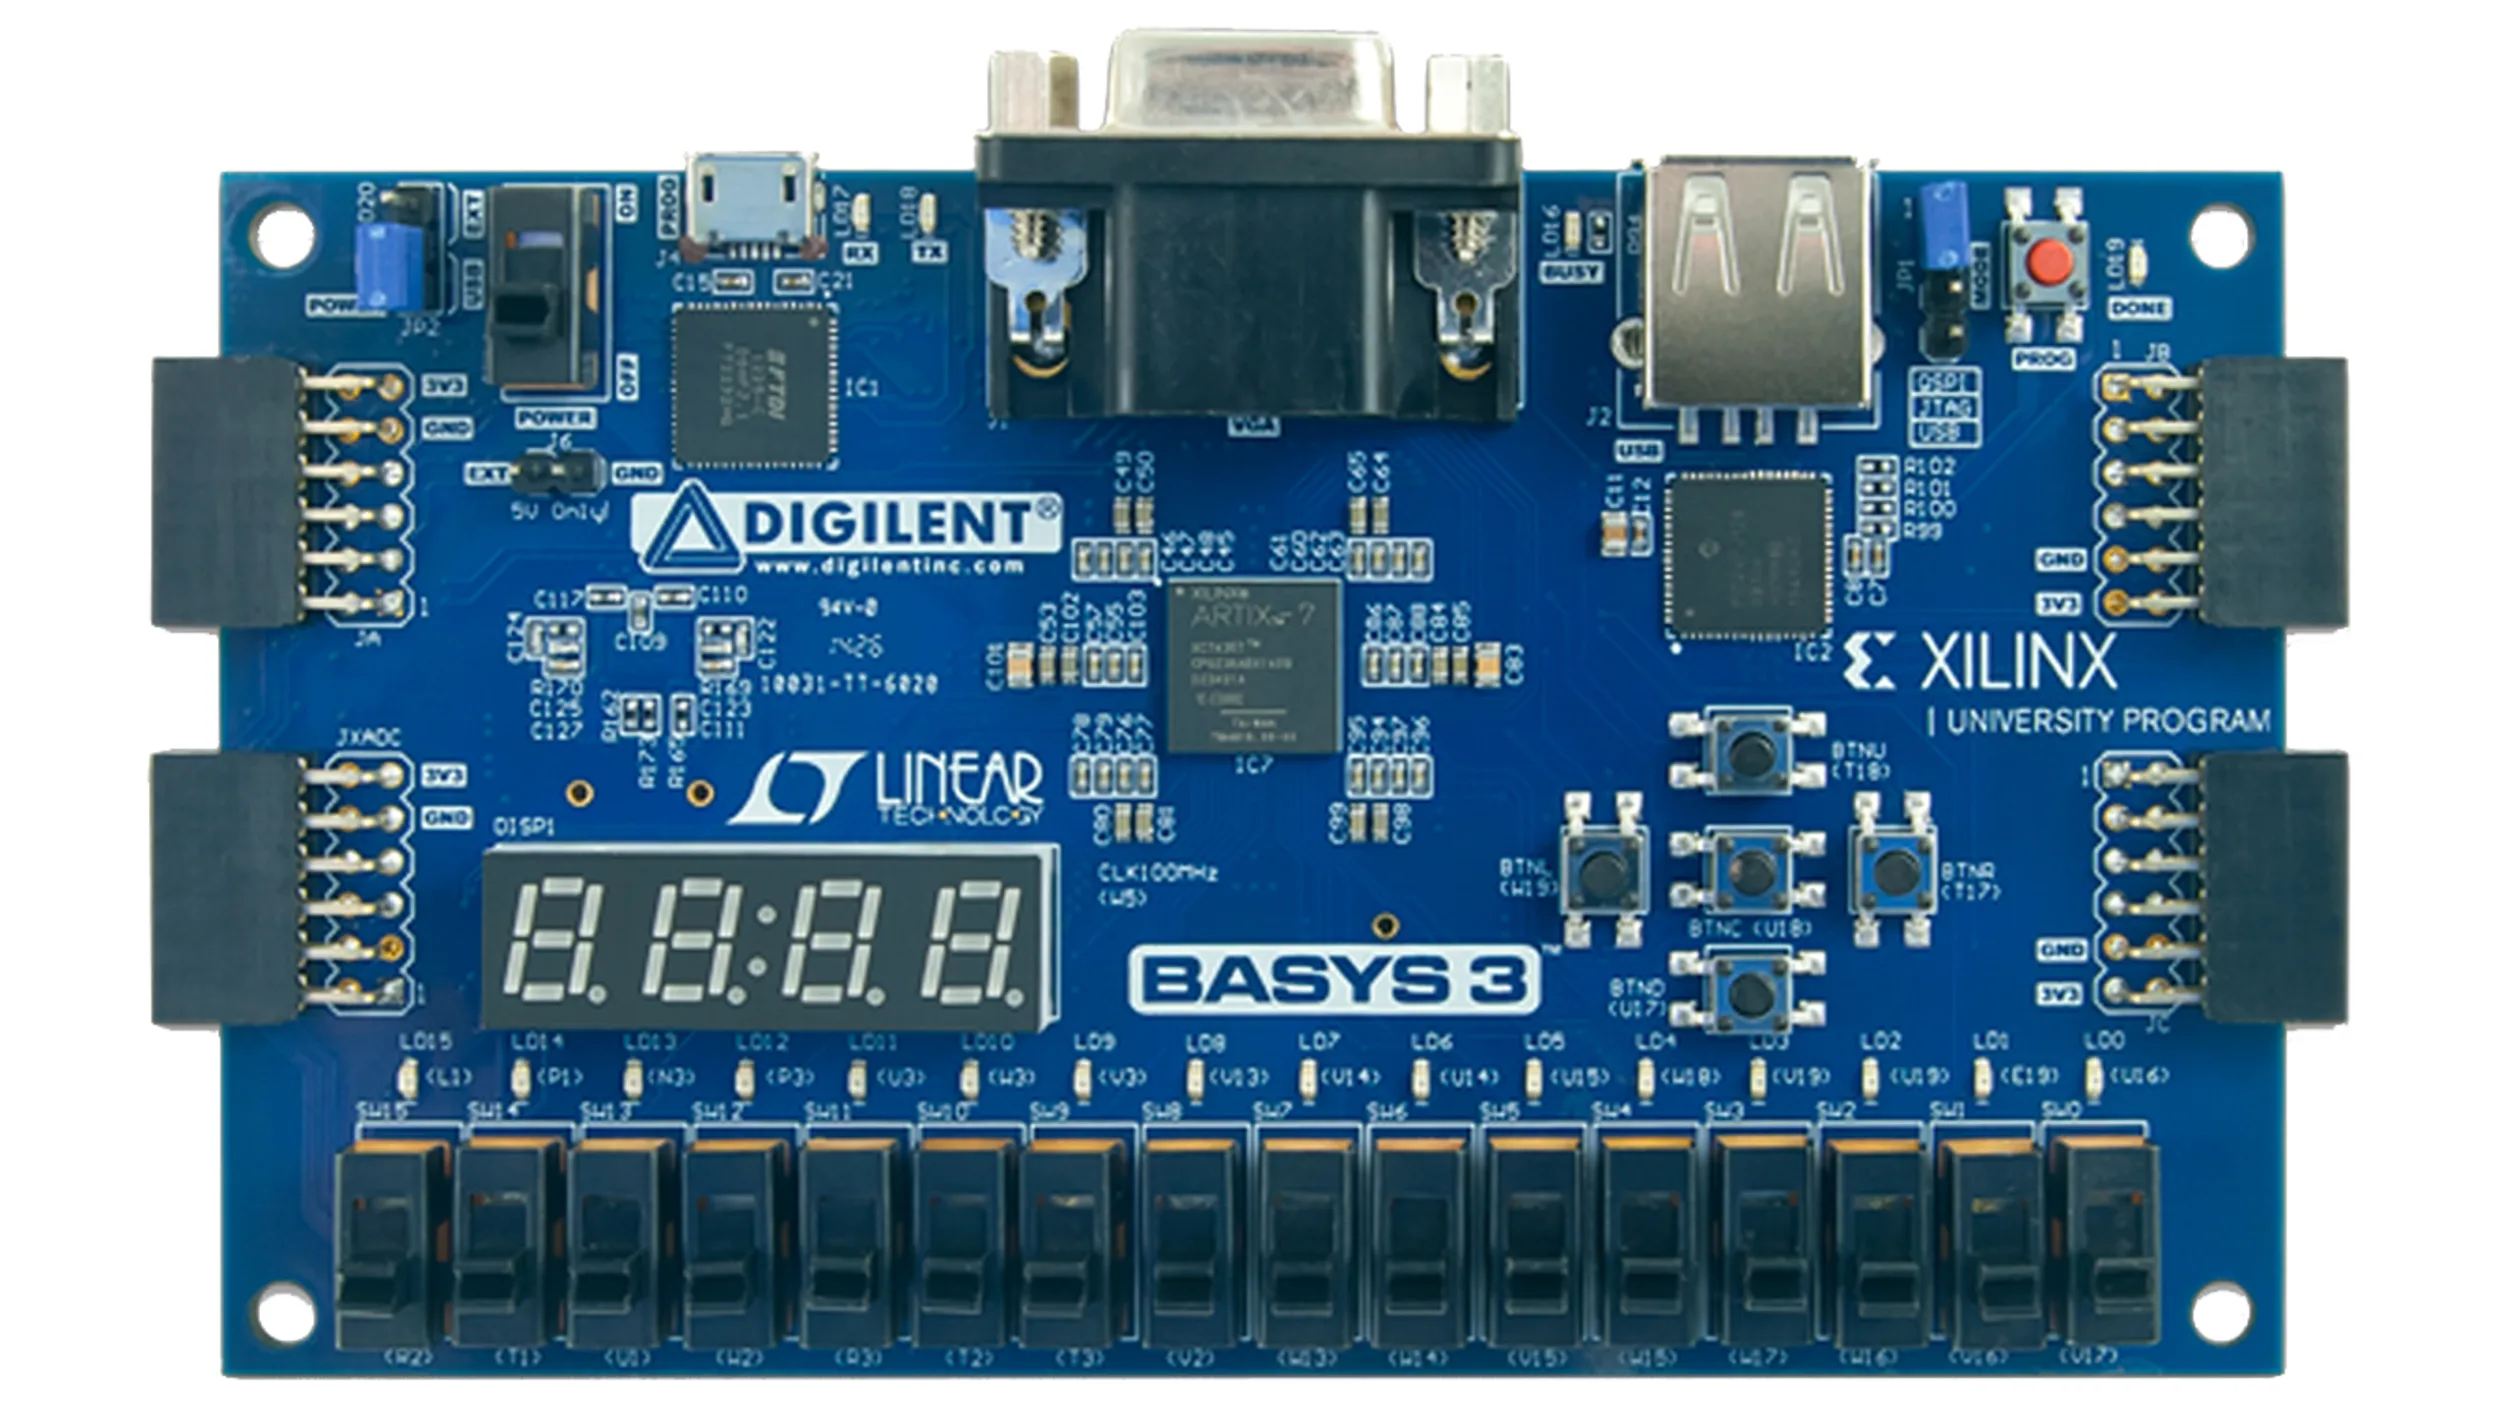
\includegraphics[width=0.65\textwidth]{basys3.png}
    \caption[Digilent Basys 3 FPGA development board]{Digilent Basys 3 FPGA development board.}
    \label{fig:dev_board}
\end{figure}

\newpage


\subsection{RISC-V Softcore}

FPGAs provide full configurability of the hardware, and offer softcore processors as a means to control the hardware.
A system on chip (SoC) is implemented on the FPGA, and is controlled by a RISC-V softcore processor which provides a method to control the hardware and run higher layer tasks, which is generally required for embedded systems being simulated here.
Fundamentally, it provides a mapping to pass data to the dedicated hardware and access the signals to retrieve the results.

The NeoRV32 softcore implementation was selected due to it's highly documented ecosystem, and personal familiarity\footnote[1]{See: https://github.com/stnolting/neorv32}.
For connecting the processor to the FPGA, the Wishbone B4 classic bus was selected due to it's high bandwidth and relatively easy implementation - as the NeoRV32 natively supports the interface.
The bus uses a 32-bit data width, as the primary use is to allow for mapping of a memory address for the accelerator to retrieve the image data from.

\subsection{Convolution}
\label{sec:convolution}

Convolution operations form the computational foundation of modern image processing algorithms and neural networks, transforming input data into higher-dimensional feature representations. In Convolutional Neural Networks (CNNs), these operations constitute approximately 90% of the total computational workload during inference [citation needed], making them the primary bottleneck in system performance.

The mathematical formulation of a 2D convolution with multiple input channels can be expressed as:

\begin{equation}
    Y(i,j) = \sum_{m=0}^{K-1} \sum_{n=0}^{K-1} \sum_{c=0}^{C-1} X(i+m,j+n,c) \cdot W(m,n,c)
\end{equation}

where $X$ represents the input feature map, $W$ represents the convolution kernel, $K$ denotes the kernel size, $C$ represents the number of input channels, and $Y$ is the resulting output feature map.

Hardware acceleration of convolution operations offers several critical advantages:

\begin{itemize}
    \item \textbf{Computational Offloading}: Dedicated FPGA hardware handles intensive convolution computations, freeing the main processor for other critical tasks
    \item \textbf{Parallel Processing}: The inherent parallelism of FPGA architectures enables concurrent execution of multiple convolution operations
    \item \textbf{Deterministic Performance}: Hardware implementation ensures consistent execution times, crucial for real-time applications
    \item \textbf{Energy Efficiency}: Dedicated hardware structures provide better performance-per-watt compared to general-purpose processors
\end{itemize}

The convolution accelerator is implemented using parameterizable hardware description language (HDL) generics, enabling compile-time optimization. This approach eliminates runtime initialization overhead and allows for application-specific tailoring. Table \ref{tab:convolution_parameters} details the key parameters governing the convolution operation for this implementation.

\begin{table}[h!]
    \centering
    \caption{Key parameters for hardware convolution implementation}
    \label{tab:convolution_parameters}
    \begin{tabular}{ccc}
        \toprule
        Parameter & Symbol & Description \\
        \midrule
        Image Size & I & Input feature map dimensions (height × width) \\
        Kernel Size & K & Convolution kernel dimensions (K × K) \\
        Input Channels & C & Number of input feature map channels \\
        Bit Width & Q & Fixed-point precision for values \\
        Output Channels & O & Number of output feature maps \\
        Stride & S & Convolution window step size \\
        Zero Padding & Z & Padding width applied to input boundaries \\
        \bottomrule
    \end{tabular}
\end{table}

The hardware architecture employs a custom type system to abstract multi-dimensional data structures. Feature maps, which represent either input images or intermediate representations, are modeled as three-dimensional matrices of pixels (height × width × channels). This abstraction is implemented through a parameterized array type that can be efficiently mapped to hardware vectors.

At the implementation level, these higher-dimensional structures are flattened into single-dimensional vectors, with careful attention to maintaining spatial relationships. This approach provides several advantages:

\begin{itemize}
    \item \textbf{Memory Efficiency}: Optimized storage and access patterns for FPGA block RAM
    \item \textbf{Hardware Mapping}: Direct correspondence between logical and physical data organization
    \item \textbf{Abstraction}: High-level interface for design and verification while maintaining low-level efficiency
\end{itemize}

\subsubsection{MAC Unit}

The Multiply-Accumulate (MAC) unit forms the fundamental computational element of the convolution operation in hardware. Each MAC unit comprises dedicated DSP blocks or equivalent arithmetic units for multiplication and cascaded adder trees for accumulation, optimized for the FPGA fabric.

The basic MAC operation for a single convolution point can be expressed as:

\begin{equation}
    y = \sum_{i=0}^{n} w_i \cdot x_i
\end{equation}

where $w_i$ represents kernel weights and $x_i$ represents input feature values.

\begin{figure}[h]
    \centering
    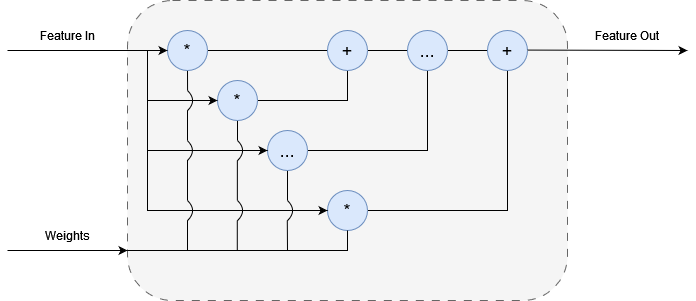
\includegraphics[width=0.75\textwidth]{mac.png}
    \caption{Hardware architecture of the MAC unit showing parallel multipliers and adder tree configuration.}
    \label{fig:mac}
\end{figure}

Resource utilization scales with the kernel dimensions according to:
\begin{equation}
    \text{DSP}_{\text{total}} = K \times K \times C
\end{equation}

where $K$ is the kernel size and $C$ is the number of input channels. 

The MAC units operate on fixed-point arithmetic to maintain precision while optimizing hardware resources, with parameterizable bit widths allowing for application-specific trade-offs between precision and resource utilization.
However, as the size of the feature map and kernel increases, the number of MAC units required increases proportionally to the kernel size.
To reduce the number of MAC units required, the concept of folding is introduced.
This is a method to reduce the number of MAC units required by sharing the MAC units across time.
This is achieved by partitioning the input data into slices which can then be pipelined through the MAC units, and as such the resources are shared across different time intervals to reduce the amount of resources required.
The following sections detail the implementation of folding for convolution to reduce the required resources.

\clearpage 
\subsubsection{No Folding}

Convolution without folding is a fully parallelised approach, whereby the entire kernel is moved across the image in a single clock cycle.
This is naturally implicit for hardware description languages, as operations are inherently performed in parallel (see listing \ref{lst:code_snippet}).

\begin{lstlisting}[style=vhdl, caption={Implementation of fully parallelised convolution}, label=lst:code_snippet]
for conv_row in feature_o'range(1) loop
    for conv_col in feature_o'range(2) loop
        for conv_chan in feature_o'range(3) loop            
            for mac_row in weights_i'range(1) loop
                for mac_col in weights_i'range(2) loop
                    for mac_chan in 1 to C loop
                        ----- ... -----
                    end loop;
                end loop;
            end loop;
        end loop;
    end loop;
end loop;
\end{lstlisting}

The operation will then be dependent on the fastest clock speed possible for the FPGA to ensure the timing constraints are met, as the additions must complete within the clock cycle.
It utilises the described MAC units in figure \ref{fig:mac} for each slice of an image, with the corresponding kernel weight slice.
This is represented by the feature map type, which represents the slicing of the image matrix.
Zero padding is applied as necessary based on the design generics at the tail and head of the image matrix, in each dimension.
The convolution process in hardware is described in figure \ref{fig:conv}.



\begin{figure}[h]
    \centering
    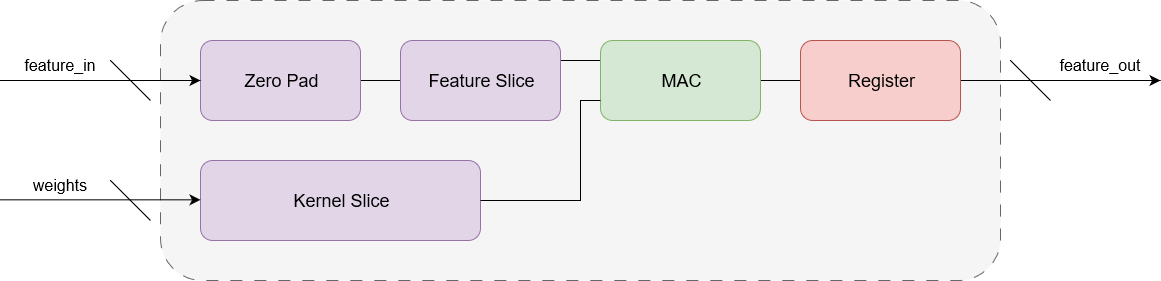
\includegraphics[width=0.75\textwidth]{conv.png}
    \caption{Convolution operation without folding.}
    \label{fig:conv}
\end{figure}


\subsubsection{Partial Folding}
A partially folded approach improves the sustainability of implementing a kernel with concern for the available hardware resources.
This is achieved by migrating to a partial dataflow approach, where the MAC units are shared across the kernel size.
It implements time multiplexing to remove the need for additional MACs based on the desired output channels.

To achieve this, an iterator is implemented to step through the values contained in the feature map and corresponding kernel weights, shown in figure \ref{fig:iterator}.
This produces a smaller slice of the image which is passed to the MAC units for processing.
It is then demultiplexed to produce the final result back as the feature map type.
This approach requires a small amount of extra logic to handle the partial slices, however, it has a marked decrease in the required resources, and as such is a more sustainable approach.

\begin{figure}[h]
    \centering
    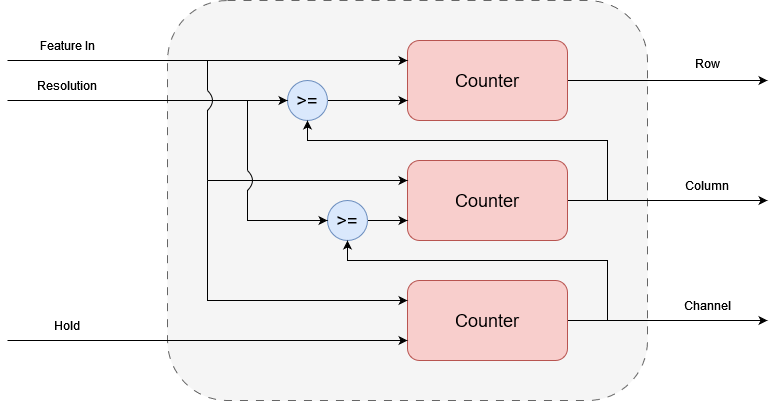
\includegraphics[width=0.75\textwidth]{iterator.png}
    \caption{Hardware representation of the MAC unit.}
    \label{fig:iterator}
\end{figure}

The fully parallelised approach can be modified to include folding by utilising the iterator to step through the feature map and kernel weights.
This is shown in figure \ref{fig:partial_folded}.

\begin{figure}[h]
    \centering
    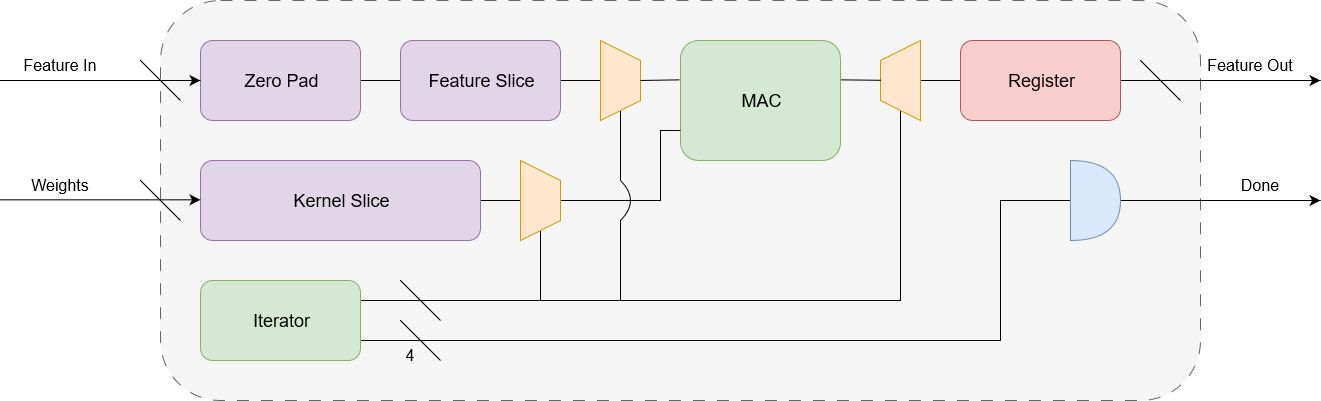
\includegraphics[width=0.75\textwidth]{conv_partially_folded.png}
    \caption{Convolution operation with partial folding via the iterator.}
    \label{fig:partial_folded}
\end{figure}



\subsubsection{Complete Folding}
A complete folding approach involves a single MAC unit that is shared across the entire image.
This will introduce a constant number of MAC units, agnostic to the kernel size.
However, the tradeoff comes at additional logic to handle the iteration of the feature map and kernel weights.

To implement the slicing of individual feature map values and kernel weights, a complete dataflow architecture is implemented.
This requires a transmit module to handle the slicing of the feature map, and a receive module to handle the slicing of the kernel weights.
These form the control unit in the form of a finite state machine to coordinate the streaming of data to the MAC unit.
As convolution requires the summation of a number of values, the receive module must store the partial results until all the values have been summed to produce the final result when the iteration is complete.
This is shown in figure \ref{fig:fully_folded}.

\begin{figure}[h]
    \centering
    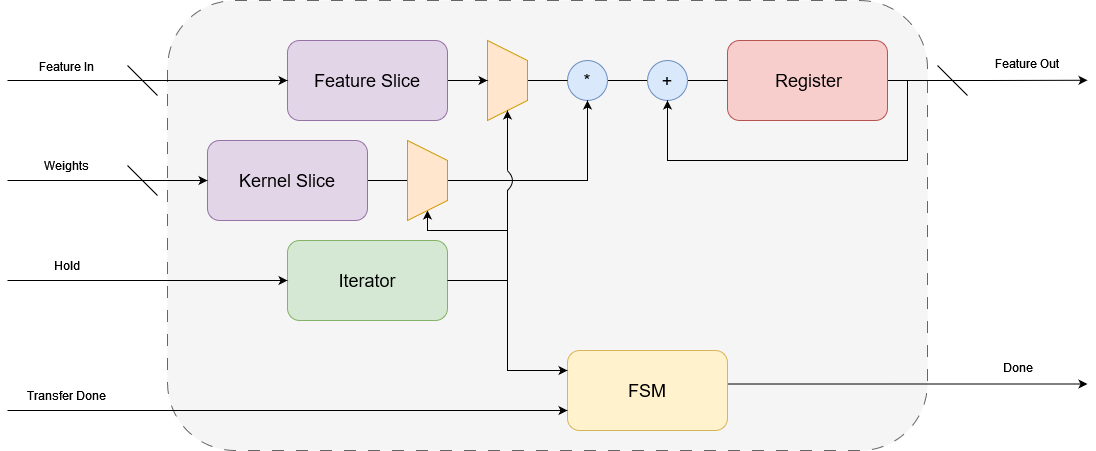
\includegraphics[width=0.75\textwidth]{fully_folded_conv.png}
    \caption{Hardware representation of the MAC unit.}
    \label{fig:fully_folded}
\end{figure}

\subsection{Activation Function}
The activation function is used to introduce non-linearity to the model, which fundamentally enables it to model complex patterns and relationships in data \cite{DCNN}. The most common activation function used in CNNs is the Rectified Linear Unit (ReLU), which is defined as:
\label{sec:relu}

\begin{equation}
    f(x) = \max(0, x)
\end{equation}

This was selected over other activation functions such as the Sigmoid and Tanh due to its computational efficiency and ease of implementation at a hardware layer \cite{10}. The hardware implementation consists of a comparator and multiplexer to select between zero and the input value, as shown in figure \ref{fig:relu}.

\begin{figure}[h]
    \centering
    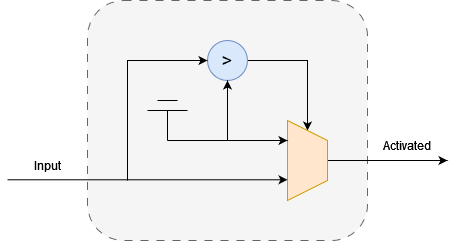
\includegraphics[width=0.65\textwidth]{relu.png}
    \caption{Hardware implementation of ReLU activation function}
    \label{fig:relu}
\end{figure}

While activation functions could be implemented as standalone modules, the ReLU implementation is integrated directly into the convolution module for several key reasons:

\begin{itemize}
    \item \textbf{Timing Efficiency}: The activation can be performed within the same clock cycle as the final MAC operation, eliminating additional pipeline stages \cite{14}
    \item \textbf{Resource Optimization}: Integration allows sharing of control signals and timing logic, reducing overall resource utilization
    \item \textbf{Reduced Complexity}: Direct integration eliminates the need for additional interface logic and buffering between modules
\end{itemize}

The hardware implementation leverages the fact that negative numbers in two's complement representation have their most significant bit (MSB) set to 1. Therefore, the comparator only needs to examine this bit to determine if the input is negative, making the implementation particularly efficient in terms of both latency and resource utilization. The multiplexer then selects either zero or the input value based on this single-bit comparison.

This architectural decision follows established principles of hardware optimization, where tightly coupled operations are combined to minimize both latency and resource usage. The marginal increase in convolution module complexity (approximately 32 LUTs per output channel) is justified by the benefits of reduced latency and simplified control logic, particularly important for resource-constrained FPGA implementations \cite{16}.

\subsection{Pooling Layer}
\label{sec:pooling}

Pooling layers are used to reduce the spatial dimensions of the feature maps while retaining important information \cite{19}. The max pooling operation is implemented using a sliding window approach, similar to convolution, but instead of multiplication and accumulation, it performs a comparison operation between values.

At a hardware level, each pooling unit consists of a comparator that determines the maximum value between two inputs. This is significantly more resource-efficient than MAC units as it only requires comparison logic. For a 2x2 pooling window with stride 2, the output dimensions are halved in both spatial dimensions, effectively reducing the computational complexity of subsequent layers \cite{10}.

The hardware implementation can be approached in two ways:
\begin{itemize}
    \item \textbf{Parallel Implementation}: All comparisons within a pooling window are performed simultaneously, requiring multiple comparator units but providing single-cycle operation
    \item \textbf{Folded Implementation}: A single comparator is time-multiplexed across the pooling window, reducing resource utilization at the cost of increased latency
\end{itemize}

As shown in figure \ref{fig:pooling_hardware}, the design implements a parallel approach for the 2x2 pooling window. This decision was made because:
\begin{itemize}
    \item The resource cost of comparators is significantly lower than MAC units
    \item Parallel implementation maintains the dataflow of the convolution output
    \item The reduced feature map size already provides significant computational savings
\end{itemize}

\begin{figure}[h]
    \centering
    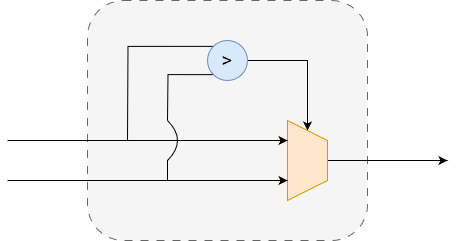
\includegraphics[width=0.75\textwidth]{pool.png}
    \caption{Hardware implementation of max pooling layer showing parallel comparator arrangement}
    \label{fig:pooling_hardware}
\end{figure}

The pooling operation can be expressed mathematically as:

\begin{equation}
    y_{i,j} = \max_{m,n \in R} x_{i+m,j+n}
\end{equation}

where $R$ represents the pooling region (2x2 in this implementation), and $(i,j)$ are the output coordinates. This operation requires significantly fewer resources than convolution while providing essential dimensionality reduction for the neural network architecture \cite{18}.

\subsection{Fully Connected Layer}
\label{sec:fully_connected}

The fully connected layer performs a matrix multiplication between the input features and the weight matrix. This operation can be decomposed into a series of dot products, which can be implemented using MAC units similar to those used in the convolution layer \cite{ResourceEfficient}. The primary difference is that fully connected layers operate on flattened 1D vectors rather than 2D feature maps.

The hardware implementation utilizes parallel MAC units to compute multiple dot products simultaneously. The number of parallel units can be configured based on available resources and desired throughput. For a layer with $N$ inputs and $M$ outputs, the operation can be expressed as:

\begin{equation}
    y_j = \sum_{i=1}^{N} w_{ij}x_i + b_j
\end{equation}

where $y_j$ is the $j$th output, $w_{ij}$ represents the weight connecting input $i$ to output $j$, $x_i$ is the $i$th input, and $b_j$ is the bias term.

Similar to the convolution layer, the fully connected layer can be implemented with different levels of folding. However, this is not explored in this implementation as it is a specific to neural network architectures and not general image processing.
It is mentioned here for completeness.

\begin{itemize}
    \item \textbf{No Folding}: Requires $N \times M$ MAC units, providing maximum throughput but highest resource utilization
    \item \textbf{Input Folding}: Time-multiplexes the input vector, requiring $M$ MAC units
    \item \textbf{Complete Folding}: Uses a single MAC unit iteratively, minimizing resource usage at the cost of increased latency
\end{itemize}

For the implemented design, input folding was selected as it provides a reasonable compromise between resource utilization and performance \cite{16}. This approach:
\begin{itemize}
    \item Reduces hardware complexity compared to full parallelization
    \item Maintains acceptable throughput for inference operations
    \item Allows for efficient resource sharing with convolution layers
    \item Simplifies control logic and data routing
\end{itemize}

The timing characteristics of the folded implementation can be determined by:

\begin{equation}
    \text{Cycles} = N + P
\end{equation}

where $N$ is the number of inputs and $P$ is the pipeline depth of the MAC unit. This demonstrates how the latency scales linearly with input size, making it suitable for resource-constrained FPGA implementations \cite{17}.

\section{Network Quantization}
\label{sec:quantization}

Quantization is essential for efficient hardware implementation of neural networks.
It reduces memory requirements and simplifies computations by converting floating-point values to fixed-point or integer representations.
The process must be carefully managed to maintain model accuracy while reducing precision.

\subsection{Training-Aware Quantization}
\label{sec:training_quantization}

To maintain accuracy while reducing precision, quantization is performed during the training process.
This allows the network to adapt its weights to compensate for the reduced precision.
The quantization process is as follows:

\begin{enumerate}
    \item Define quantization parameters (bit width, scaling factors)
    \item Forward pass with quantized weights and activations
    \item Backward pass with straight-through estimator
    \item Update full-precision weights
    \item Quantize updated weights
\end{enumerate}

The quantization function Q(x) for an n-bit fixed-point representation is defined as:

\begin{equation}
    Q(x) = \text{round}(x \cdot 2^n) \cdot 2^{-n}
\end{equation}

For the design, the network is quantized in training to utilise an 8-bit integer representation.
This is effectively analogous to using a fixed-point representation, with the scaling factor being $2^8$, which is recommendation for future work to better generalise the layers developed.

\section{Neural Network Implementation}

\subsection{Dataset}
As part of the design, a dataset of images was required to demonstrate recognition capabilities of the accelerator built on top of the convolutional core.
Digit-based datasets, such as MNIST, are commonly used for demonstrating the capabilities of CNNs and are therefore used for this project.
The digit dataset used in this project consists of a down-sampled version of MNIST, with each image being 8x8 pixels in size using a single colour channel represented in 8-bit greyscale.
This is due to the resource limitations of the development board used, and to lower the time required for synthesis.
As the network is implemented at a hardware level, increasing the scale of the image is directly commensurate with the required resources and also training time.
A sample image of the dataset can be seen in figure \ref{fig:digit_dataset}.

\begin{figure}[h]
    \centering
    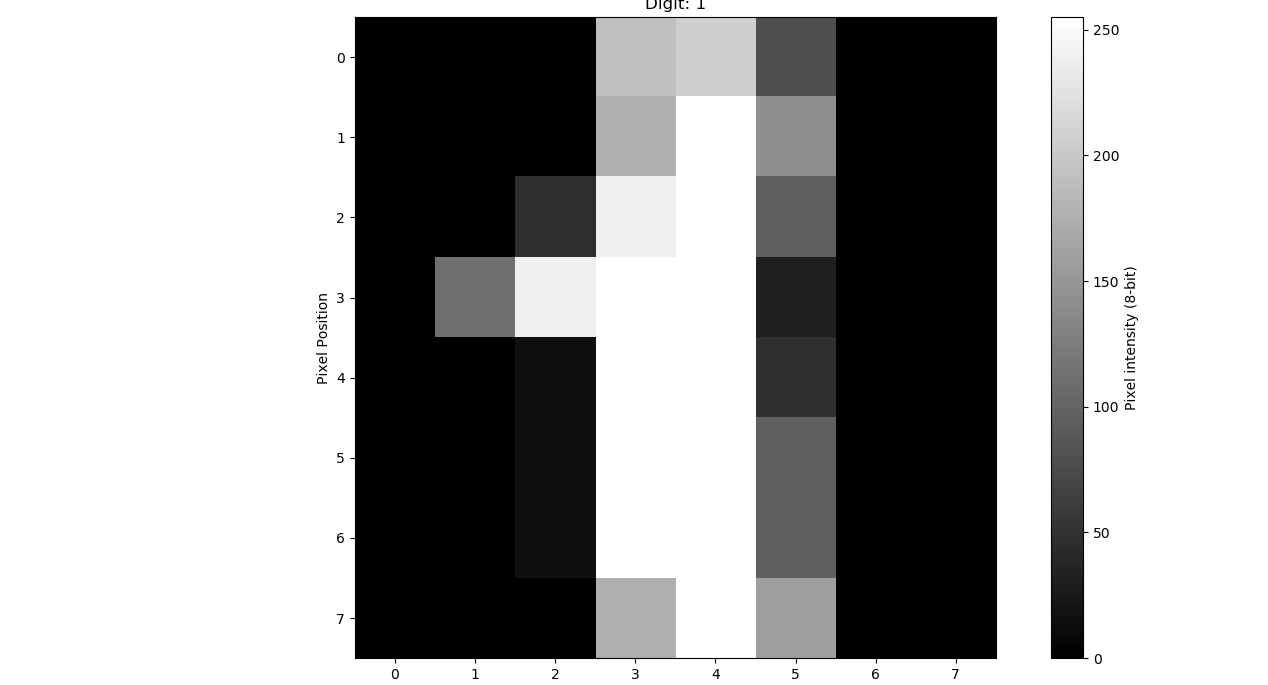
\includegraphics[width=0.5\textwidth]{digit.png}
    \caption{Sample images from the downsampled MNIST dataset used for training and inference}
    \label{fig:digit_dataset}
\end{figure}

\subsection{Model}
A convolutional neural network was trained in software with inference to be performed on the hardware accelerator.
The architecture selected is effectively the simplest possible CNN architecture to demonstrate the feasibility of the design.
It consists of a single convolutional layer, with a max pooling to downsample the data followed by a fully connected layer to classify the data.
The model description is shown in figure \ref{fig:model_architecture}.

\begin{figure}[h!]
    \centering
    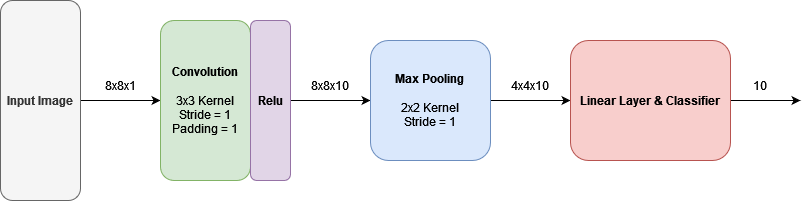
\includegraphics[width=0.65\textwidth]{model.png}
    \caption[Model architecture]{Model architecture.}
    \label{fig:model_architecture}
\end{figure}

The model was trained using an 80/20 split of the dataset, with 80\% used for training and 20\% used for validation.
The model was trained for 20 epochs with a batch size of 32.
As it is a classification problem, cross entropy loss was used as the loss function with an Adam optimiser to reduce the need for configuring learning rates.
It demonstrated an accuracy of 87\% on the validation set.
A summary of the network parameters can be seen in table \ref{tab:network_parameters}.
This is not discussed in detail as it is not central to the thesis, and is provided as reference for completeness.

\begin{table}[h!]
    \centering
    \caption{Summary of the network parameters.}
    \label{tab:network_parameters}
    \begin{tabular}{ccc}
        \toprule
        Parameter & Value & Description \\
        \midrule
        Loss function & Cross Entropy & Measure of accuracy \\
        Optimiser & Adam & Adaptive learning rate \\
        Batch Size & 32 & Number of samples per batch for training \\
        Epochs & 20 & Number of iterations to train the model \\
        Classes & 10 & Number of classes to classify as the output\\
        \bottomrule
    \end{tabular}
\end{table}

\subsection{Machine Learning Core}
The produced generic layers can be assembled to create a complete neural network, with a direct mapping from a software model.
There are two fundamental choices to be made when assembling the network:

\begin{enumerate}
    \item A streaming approach, where the next layer is loaded while the current layer is being processed
    \item A sequential approach, where each layer is processed in order
\end{enumerate}

Streaming architectures are typically more efficient in terms of resource utilisation, as they are non-blocking approaches.
The layers will have the outputs streamed to the following operation, while new input data is loaded into the current layer.
This fundamentally ensures that the layers are always fully utilised, and as such the resource utilisation of the design is minimised and can improve the latency.

A sequential approach is a single engine which executes the layers in order, and as such the resource utilisation is higher.
However, it is simpler to implement, and as such is more amenable to assembly from generic blocks.
It requires a single control block, via a FSM, to manage the dataflow between layers.
This makes it more extensible and flexible, but at the cost of increased resource utilisation and performance.
However, due to the simplicity of the design, it is the approach selected for this implementation.
This approach is shown in figure \ref{fig:ml_core}.

\begin{figure}[h]
    \centering
    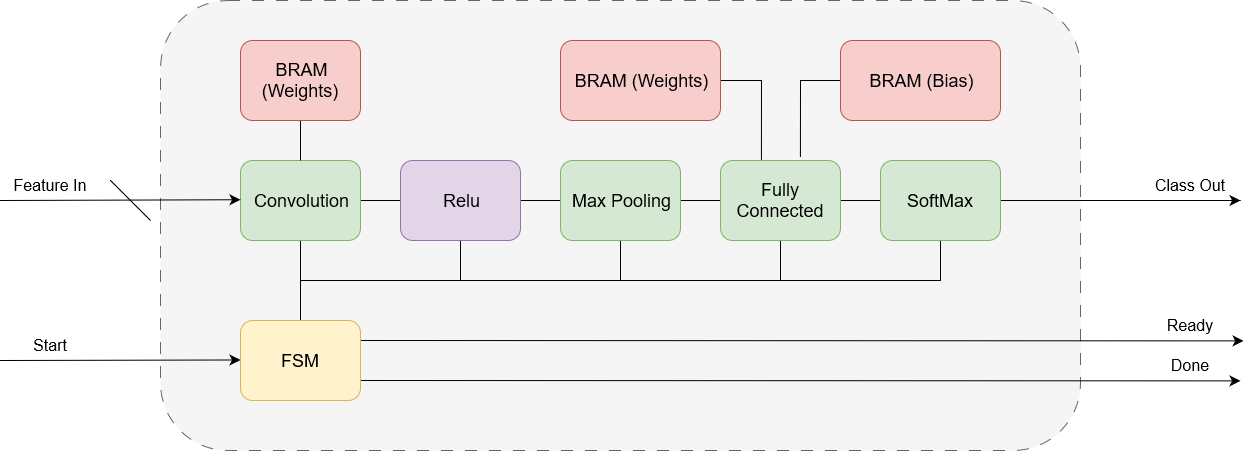
\includegraphics[width=0.75\textwidth]{ml_core.png}
    \caption{Hardware representation of the MAC unit.}
    \label{fig:ml_core}
\end{figure}

The machine learning core represents an assembly of the generic layers to form a complete neural network accessible via a memory mapped interface, using embedded network parameters at synthesis.
As discussed, a sequential architecture was selected due to the ability to implement virtually any network using the given components.
The core is controlled by a control unit, implemented as a finite state machine, to manage the dataflow between layers.
This is a relatively simple implementation, but provides a means to implement a wide range of networks with ease.
